\documentclass{../../tex_template/asaproc}
\usepackage{graphicx} % \includegraphics
\usepackage{float}    % To keep figures in right place. 
                      % Usage: \being{figure}[H] \includegraphics{tmp.pdf} \end{figure}
\usepackage{subfig}   % \subfloat
\usepackage{amsmath}  % bmatrix, pmatrix, etc
\usepackage{bm}
\newcommand{\p}[1]{\left(#1\right)}
\newcommand{\bk}[1]{\left[#1\right]}
\newcommand{\bc}[1]{ \left\{#1\right\} }
\newcommand{\abs}[1]{ \left|#1\right| }
\newcommand{\norm}[1]{ \left|\left|#1\right|\right| }
\newcommand{\E}{ \text{E} }
\newcommand{\N}{ \mathcal N }
\newcommand{\ds}{ \displaystyle }

%\usepackage{times}
%If you have times installed on your system, please
%uncomment the line above

%For figures and tables to stretch across two columns
%use \begin{figure*} \end{figure*} and
%\begin{table*}\end{table*}
% please place figures & tables as close as possible
% to text references

\newcommand{\be}{\begin{equation}}
\newcommand{\ee}{\end{equation}}
\newcommand{\y}{\bm y}
\newcommand{\X}{\bm X}
\newcommand{\Xb}{\bm {X\beta}}
\newcommand{\bh}{\bm{\hat\beta}}
\newcommand{\XXi}{(\X^T\X)^{-1}}
\newcommand{\M}{\mathcal{M}}

\title{FYE--- Ozone}

%input all authors' names
\author{
  Test ID: 701$^1$\\
  University California -- Santa Cruz$^1$\\
}

%input affiliations
%{USDA Forest Service Forest Products Laboratory}

\begin{document}
\maketitle
\begin{abstract}
Exposure to high ozone levels is known to be associated with the development
of respiratory and other illnesses. Hence, modeling ozone levels is of interest
to climatoligists and medical professionals. The effects on ozone levels by
temperature, wind speed and radiation are explored using a g-prior in this 
paper. The results of the analysis show that all three of these variables are
important in predicting ozone concentrations. In addition, a model with
radiation as a covariate substantially the Bayes factor beyond the model
that does not include radiation.

\begin{keywords}
Bayesian Regression, ozone, temperature, wind speed, radiation, g-priors
\end{keywords}
\end{abstract}

\section{Introduction}
Exposure to high ozone levels is known to be associated with the development of
respiratory and other illnesses. Ozone levels are typically measured in terms
of concentration (parts per billion or simply ppb). Ozone levels of 70ppb are
considered high or dangerous. Hence, modeling ozone levels is an area of 
concern to medical professionals, scientists, as well as governments. In this
study, the effects of radiation (0 for low, 1 for moderate to high levels), 
temperature (F$^\circ$), and wind speed (mph) are explored using a Bayesian
regression model which makes use of Zellner's g-prior as the prior for covariates
in the model. Of particular interest in this paper is whether including the 
radiation variable in the model improves the model that does not include it.
Using a g-prior-based regression model, computing the Bayes factors for competing
models becomes simple.\\

This remainder of this paper is divided into 4 parts. The first part is an 
exploratory analysis of the data. The next part outlines the methods used in
the analysis and model fitting. This section will include a brief overview
of Zellner's g-prior. The next section contains the results of the analysis.
The final section contains concluding remarks and items for future studies.

\section{Exploratory Analysis}
The data provided consists of 111 rows (observations) and 4 columns -- the
first column being ozone concentration, and the remaining columns being the
values corresponding to each of the aforementioned variables. The data is
plotted as a scatter plot matrix as shown in Figure \ref{fig:pairs} Along the
diagonal are the univariate histograms for each of the variables. Displayed in the
lower traingle are the correlations between each pairs of covariates. (The 
value .464 corresponds to the correlation between ozone and radiation, etc.)
The upper triangle displays the scatter plot for each pair of variables.\\

\begin{figure}[H]
  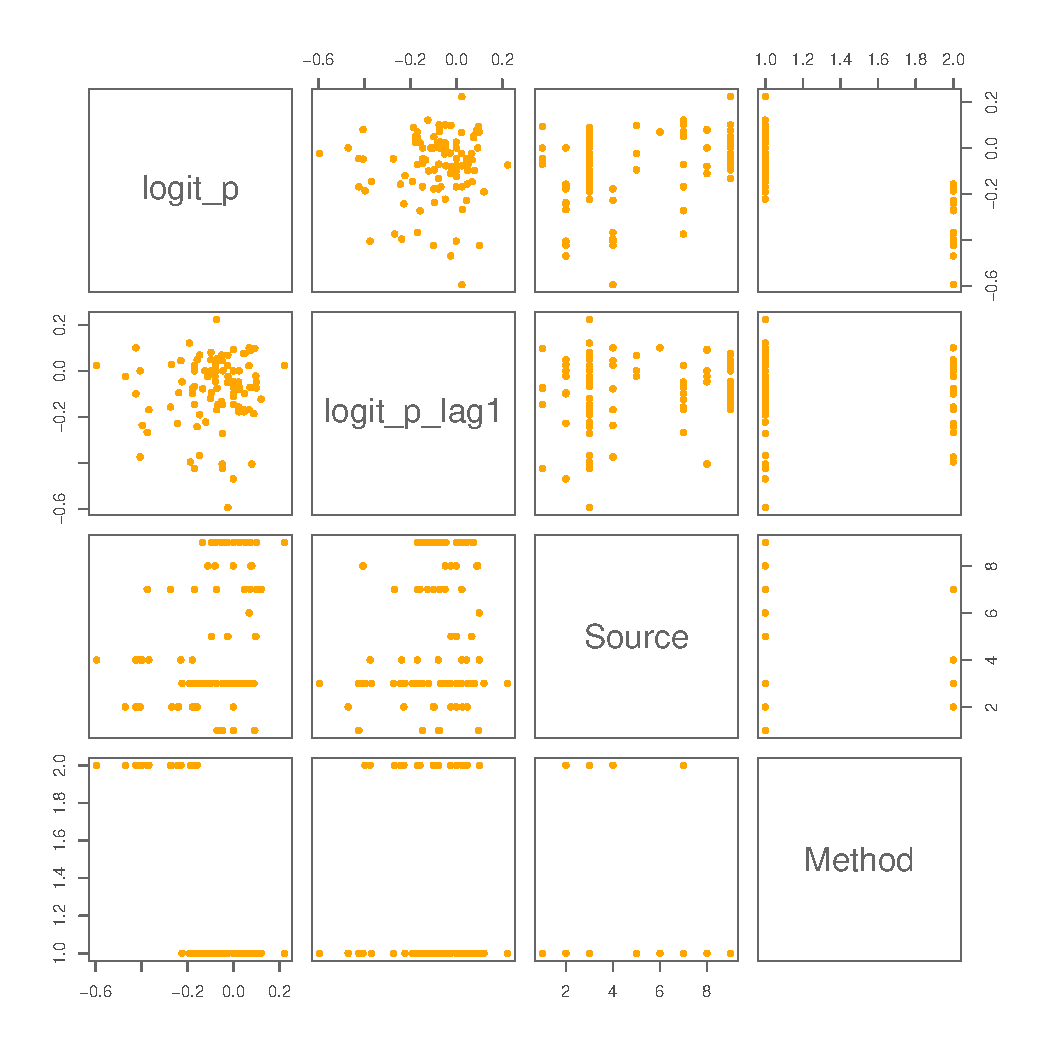
\includegraphics[scale=.5]{figs/pairs.pdf}
  \caption{\small Scatter plot matrix of ... }
  \label{fig:pairs}
\end{figure}

A first observation is that ozone concentrations appear non-linearly related to
all of the variables. To exploit the simplicity of linear models, a log
transform is imposed on ozone concentrations. The resulting data is shown in
Figure \ref{fig:logpairs}. After the transformation, the data indeed exhibit a
linear trend between ozone and the other variables. Another item to note is
that the variables are at most moderately linearly correlated with one another.
(Ozone and temperature have the largest correlation of .75.) This is a
desireable property in regression models as high correlation between covariates
often leads to inflated variances of the estimated coefficients. Also note that
the range for each variable is very different. Log-ozone ranges from 0 to 5.12,
radiation is a binary variable, temperatures range from 57 to 97 F$\circ$, and
wind speeds range from 2.3 to 20.7 mph. Taking this variability in ranges into
consideration, it may be appropriate to center and scale the variables while
doing a regression analysis. For simplicity, this step is omitted.

\begin{figure}[H]
  \includegraphics[scale=.5]{figs/log_ozone_pairs.pdf}
  \caption{\small Scatter plot matrix of ... }
  \label{fig:logpairs}
\end{figure}

Given this preliminary analysis, a good candidate linear model is that with
response variable $\y$ being the log ozone concentration, and covariates being
radiation level, temperature, and wind speed. This is a good candidate model
because log-ozone concentration is linear with the covariates and the 
covariates are not strongly correlated.

\section{Methods}
The linear model used in this analysis is a Bayesian linear regression model
using Zellner's g-prior for the covariates. As mentioned, this model is both
simple to fit, and provides easy diagnostics for model comparison using 
Bayes factors. A review of the mechanics of this model is provided here.\\

A regression model that uses g-priors is typically specified as follows:
\[
  \begin{array}{rclcl}
    \y &|& \X,\bm\beta,\phi &\sim& \mathcal{N}_n\p{\Xb,\frac{1}{\phi}\bm I_n} \\
       && p(\bm\beta,\phi) &\propto& \frac{1}{\phi} \mathcal{N}_k (\bm 0, \frac{g}{\phi} (\X^T\X)^{-1})\\
  \end{array}
\]
where $\X$ is the matrix of covariates with a column of ones in prepended, $\y$
is the response variable, $\phi$ is the model precision, $n$ is the number of
observations, $k$ is the number of covariates, and $g$ is a constant to be
determined. There are many ways to determine a good choice for $g$ but should
typically be chosen to be large. In this study $g$ is to set be $n$. Note that
this prior is non-informative, but yields a proper posterior. \\

Given this fully specified model, the full conditional for $\bm\beta$ and
the marginal posterior for $\phi$ can be derived in closed form. They are:
\[
  \begin{array}{rclcl}
    \bm\beta &|& \y,\X,\phi &\sim& \mathcal{N}_k\p{\frac{g}{g+1}\bh, \frac{g}{(g+1)\phi} \XXi}\\
    \phi &|& \y,\X &\sim& \mathcal{G}\p{\frac{n-1}{2},\frac{n-k}{2}\hat\sigma^2+\frac{\bh^T\X^T\X\bh}{2(1+g)}}\\
  \end{array}
\]
where $\bh = \XXi\X^T\y$ and $(n-k) \hat\sigma^2 = (\y-\X\bh)^T(\y-\X\bh)$. 
(Note that here the parameterization of the Gamma distribution is shape and
rate.) Obtaining posterior samples for $\bm\beta$ and $\phi$ then becomes a
matter of simply sampling from the posterior distribution of $\phi$ and then
using the sampled values for $\phi$ to sample from the full conditional of 
$\bm\beta$. \\

Model compairson can similarly be done in a computationally efficient way using
Bayes factors. Notationally, $\M_\gamma$ will denote model $\gamma$, and
BF($\gamma,\gamma'$) will denote the bayes factor in facor of $\M_\gamma$ with
respect to $\M_{\gamma'}$, which is
$\frac{p(\y|\M_\gamma)}{p(\y|\M_{\gamma'})}$. Moreover,
the null model (with only the intercept) is denoted by $\M_{0}$. Conveniently,
the Bayes factor of model $\M_\gamma$ with respect to the null model is
computed as: \\
\[
  \text{BF}(\gamma,0) = (1+g)^{(n-p_\gamma-1)/2} (1+g(1-R^2_\gamma))^{-(n-1)/2},
\]
where $p_\gamma$ is the number of covariates in model $\gamma$, and $R^2_\gamma$
is the coefficient of determination defined as 
\[
  R^2 = \frac{\y^T(\bm {P_x-P_1})\y}{\y^T(\bm {I-P_1})\y}
\]
with $P_x$ and $P_1$ being the projection matrices onto the column space
of $\X$ and the intercept column respectively. Comparing all models
to the null model provides a method to rank models with respect to a 
resonable baseline model. Those with a high BF are preferred. Comparing 
pairs of models in isolation by taking the ratio of the BF's each
with respect to the null model. That is BF($\gamma,\gamma'$) = 
$\frac{\text{BF}(\gamma,0)}{\text{BF}(\gamma',0)}$.\\

This concludes the review of Zellner's g-prior. In the following 
analysis, two models will be fit. The first model ignores the radiation
binary variable. The second model uses all the variables. Both models
will be fit using g-priors and the two models will be compared to
each other. In both cases, the data were first split into a testing
set comprising 33 observations selected at random and a training 
set comprising the remaining 78 observations. The models are
only fit to the training set. The testing set is used only for
model checking.

\section{Analysis}
The first model is fit to the training data using only temperature and wind
speed as covariates. This model will be referred to as $\M_1$. Figure 
\ref{fig:posts1} shows the posterior for $\phi$ and $\bm\beta$.
The univariate posteriors are plotted on the diagonals, the correlations
are shown in the lower triangle, and the bivariate posteriors for each 
pair of variables are plotted in the upper triangle.
\begin{figure}[H]
  \includegraphics[scale=.5]{figs/posts1.pdf}
  \caption{\small Posteriors of ... }
  \label{fig:posts1}
\end{figure}
Shaded in navy blue are the 95\% HPD's of the univariate posteriors.
The red line shows their posterior means. The HPD of only the intercept
coefficient contains 0. This suggests that the model could possibly
do without the intercept. All the other variables are probabilistically
far from 0. \\

The second model $\M_2$ presented here contains $\M_1$ and adds the radiation
variable. Similarly to Figure \ref{fig:posts1}, Figure \ref{fig:posts2} shows
the posterior for $\phi$ and $\bm\beta$.
\begin{figure}[H]
  \includegraphics[scale=.5]{figs/posts2.pdf}
  \caption{\small Posteriors of ... }
  \label{fig:posts2}
\end{figure}
The posteriors for the coefficients of $\phi$, temperature, and wind speed
did not change much from $\M_1$. However, the posterior for the intercept changed
from having an mean of -1.02 in $\M_1$ to a mean of -.61 in $\M_2$. Still, the
HPD of the intercept in $\M_2$ contains 0. Radiation, however, was probabilistically
far from 0. The posterior mean for the coefficient for radiation is .53. \\

One way to visually assess model fit is to plot the observed data vs.
model-fitted values for log ozone levels. In Figure \ref{fig:obsvsfit}
the fitted values of log ozone concentrations using the testing set are plot
against the observed values of log ozone concentrations in the testing set.
That is, for each model, the posterior predictive distributions for new observations
$\y^*$ were produced by evaluating the model using the testing data as the covariates,
and the posterior samples for $\bm\beta$ and $\phi$ as the coefficients and precision
factor. The posterior predictive means are plotted as circles and the vertical lines
are the 95\% HPD's for each predicted observation. Furthermore, the red markers 
are associated with the model with radiation, and the blue markers are associated with
the model without radiation. Note that if the model fits the data perfectly,
all the circles should fall exactly on the diagonal line (the line that passes
through the intercept having slope 1).\\

\begin{figure}[H]
  \includegraphics[scale=.5]{figs/obsvsfit.pdf}
  \caption{\small Posteriors of observed vs. fitted. }
  \label{fig:obsvsfit}
\end{figure}

Visually, the two models behave similarly because the red and blue markers tend
to appear at about the same predicted value for each observation. Their HPD's
contain one another always. Moreover, $\M_1$ has a coverage of 27\% and $\M_2$ has
a coverage of 33\% (based on the testing set). Based on coverage, $\M_2$ is superior
to $\M_1$ in terms of predicting.\\

Since there are only 33 observations in the testing set, assessing the model
fits using a different metric may be more suitable. The root mean squared error
(RMSE) posterior distributions for each model are plotted in Figure
\ref{fig:rmse}. The RMSE for each model is computed using the average sum of
squared differences between the observed and predicted values. Smaller RMSE's
imply better model fit. The blue density represents the model without
radiation, and the red density represents the model with radiation.  The
probability that the RMSE of $\M_2$ is less than that of $\M_1$ was
approximated by computing the number of times the posterior samples in the RMSE
for $\M_2$ were greater than that of $\M_1$, and was computed to be 84\%.
This result suggests that the RMSE of $\M_2$ is usually lower, and hence, that
model 2 usually provides a better model fit.
\begin{figure}[H]
  \includegraphics[scale=.5]{figs/rmse.pdf}
  \caption{\small Posteriors of RMSE. The model with radiation has lower RMSE.
    The probability that the RMSE in the model with radiation as a coavariate
    is lower than that of the model without radiation is 84\%.}
  \label{fig:rmse}
\end{figure}

Finally, for completeness, the log Bayes factors for each model were computed
as to be log(BF(1,0)) = 34.52, log(BF(2,0)) =  40.40, and log(BF(2,1)) = 6.18.
a log$_e$ Bayes factor of 4.6 usually indicates decisive support of one model
over another. In this case, each of the models are preferred over the null
model. And model 2 is decisively favored over model 1. \\

One more helpful visual is presented in Figure \ref{fig:map}.  The axes in each
of these plots are wind speed against temperature. At each coordinate on the
plots, the log ozone levels are indicated by the redness at that coordinate.
White areas are those with less than 2.5 log ozone ppm (or 12 ozone ppm).  Dark
red areas are those with greater than 4.2 log ozone ppm (or 70 ozone ppm which
is considered dangerous). In the top subplot, the model without radiation is plot.
The full data (consisting 111 observations) are superimposed on the plot.
In general, the model is consistent with the model. Also, at high temperatures
and low wind speeds, ozone levels are higher. The next two plots are representations
for the model with radiation. The middle subplot plots the predicted ozone levels
when the radiation level is low (having a value of 0), and the
bottom subplot represents the predicted ozone levels when the radiation level is 
moderate to high (having a value of 1). Note that the ozone levels are compounded
when radiation is moderate to high. This can be seen from the trend that
the red region spans more of the area of the plot in the model with radiation,
when radiation is 1 (in the bottom plot). This suggests that the most dangerous
combination of variables in are low wind speed, high temperatures, and moderate
to high radiation levels.

\begin{figure}[H]
  \includegraphics[scale=.5]{figs/map.pdf}
  \caption{\small Heatmap of ...}
  \label{fig:map}
\end{figure}

%\begin{figure}[H]
%  \includegraphics[scale=.5]{figs/marginal.pdf}
%  \caption{\small Marginal Posterior}
%  \label{fig:marginal}
%\end{figure}

\section{Conclusions}
Zellner's g-prior is a useful tool for Bayesian linear regression. Sampling
from the posterior distribution of the covariate coefficients is
computationally simple and computation of the Bayes factors to compare models
can be done in closed form. In this analysis, the model that incorporates radiation
performs better according to several metrics, including Bayes factors. The most
dangerous combination of weather elements are high temperatures, low wind speeds, and
moderate to high radiation. These weather elements are associated with high ozone 
levels. Radiation should be included in modeling ozone, along with temperature and
wind speed. 

\begin{references}
{\footnotesize
\itemsep=3pt
\item {\em Zellner, Arnold. On assessing prior distributions and Bayesian regression analysis with g-prior distributions. Bayesian inference and decision techniques: Essays in Honor of Bruno De Finetti 6 (1986): 233-243.}
\item {\em Gelman, A., Carlin, J. B., Stern, H. S., \& Rubin, D. B. (2014). Bayesian data analysis (Vol. 2). Boca Raton, FL, USA: Chapman \& Hall/CRC, 73.}
}
\end{references}

\end{document}

%\begin{figure*}
%  \centering
%  \includegraphics[scale=.55]{figs/mapDat.pdf}
%  \vspace{-7em}
%  \caption{\small Some Caption.}
%  \label{fig:mapDat}
%\end{figure*}

%\begin{figure}[H]
%  \includegraphics[scale=.5]{figs/pairsLogRate.pdf}
%  \caption{\small Hi Motor vehicle theft is not strongly correlated with any other thefts.}
%  \label{fig:logOdds}
%\end{figure}
